\documentclass{mldsmsc}

\title{Deep Reinforcement Learning for Ad Personalization}
\author{Martin Bat\v{e}k}
\CID{00951537}
\supervisor{Mikko Pakkanen}
\date{2 September 2024}
%For today's date, use:
%\date{\today}
\logoimg{}


% THIS IS WHERE NEW COMMANDS CAN BE DEFINED
% commands below only used in the proof; otherwise can be deleted
\newcommand{\consta}{a}
\newcommand{\X}{X}
\newcommand{\EE}[1]{ \mathrm{E} [ #1 ] }
\newcommand{\inparenth}[1]{\left( #1 \right)}

\begin{document}

% Generates the Title Page
\maketitle


% Generates plagiarism declaration
\declarationname{Martin Bat\v{e}k}
\declarationdate{17 July 2024}
\declaration 


\begin{abstract}
    ABSTRACT GOES HERE
\end{abstract}

\begin{acknowledgements}
    ANY ACKNOWLEDGEMENTS GO HERE
\end{acknowledgements}

% add glossary?

% table of contents
\tableofcontents

% VERY IMPORTANT
% This command switches from Roman to Arabic numbering for main part of thesis
\mainmatter


\chapter{Introduction}

The global digital advertising market is worth approximately \$602 billion today. Due to the increasing rate of of online participation since the 
COVID-19 pandemic, this number has been rapidly increasing and is expected to reach \$871 billion by the end of 2027 \citep{RefWorks:emarketer2023digital}.
Many of the of the major Ad platforms such as Google, Facebook and Amazon operate on a cost-per-user-engagement pricing model, which usually means that 
advertisers get charged for every time a user clicks on an advertisment. This means that these platforms are incentivized to make sure that the content 
shown to each user is as relevent as possible in order to maximize the number of clicks in the long term. Attaining accurate Click-Through Rate (CTR) 
prediction is a necessary first step for Ad persionalization, which is why study of CTR prediction methods have been an extremely active part of 
Machine Learning research over the past through years.

Initially, shallow prediction methods such as Logistic Regression, Factorization Machines \citep{RefWorks:rendle2010factorization} and Field-Aware Factorization 
Machines \citep{RefWorks:juan2016field-aware} have been used for CTR prediction. However, these methods have often been shown to be unable to capture the 
higher order feature interactions in the sparse multi-value categorical Ad Marketplace datasets \citep{RefWorks:zhang2021deep}. Since then, Deep Learning methods have been 
shown to show superior predictive ability on these datasets. A number of Deep Learning models have been proposed, each using a
different techniques for feature interaction modelling, ranging from Deep Learning extensions of Factorization Machines
such as DeepFM \citep{RefWorks:guo2017deepfm:}, to novel methods such as AutoInt \citep{RefWorks:song2019autoint}. By employing a
multi-towered neural network architecture, these models are able to capture both low-order and high-order feature interactions in the data,
and therefore tend to achieve supperior predictive performance to their shallow counterparts.

However, irrespective of how well these models perform in a static environments, the reality is that user preferences
and advertisment characteristics are constantly changing. Like most online reccomender systems,
Ad personalization models must be able to adapt to these changes in order to continue to provide accurate predictions 
over the longer period \citep{RefWorks:zheng2018drn:}. This problem necessitates the use
of Reinforcement Learning for Ad personalization.

Reinforcement Learning is a subdomain of Machine Learning in which the goal is for an agent to
learn an optimal policy that maximizes the expected reward in an environment where the
state-action-reward progression can be modelled as a Markov Decision Process
\citep{puterman2014markov}. Early Reinforcement Learning methods involved 
deriving a the transition probabilities for the state-action pairs on the basis of interactions
with the environment and then using Dynamic Programming methods such as the Upper Confidence
Bound RL (UCBRL) algorith \citep{RefWorks:auer2008near-optimal}

In this report, I aim to construct a Deep Reinforcement Learning model for Ad personalization that is able to adapt to the changeing user preferences
and advertisment characteristics available on the platform. In chapter~\ref{chap:background}, I begin by providing a background to the problem
of Click-Through Rate prediction in the context of Ad personalization, and explore the unique challenges posed by the typically sparse multi-value
categorical datasets that are common in the Ad marketplace. I then proceed to review the literature on Deep Learning models for CTR prediction, highlighting
the different techniques that each framework uses to capture the key feature interactions in the data. I also review the literature on Deep Reinforcement
Learning and its applications across different domains. In chapter \ref{chap:deep-ctr-model-evaluation}, I evaluate the performance of different
Deep Learning models for CTR prediction on three well-known benchmark datasets, Criteo \citep{RefWorks:tien2014display}, KDD12 \citep{RefWorks:aden2012kdd} 
and Avazu \citep{RefWorks:wang2014click-through}. In chapter~\ref{chap:deep-rl-for-ad-personalization}, I construct a Deep Reinforcement Learning model for Ad personalization and evaluate its performance
on the same benchmark datasets. Finally, in chapter~\ref{chap:discussion}, I discuss the results of the experiments and provide some concluding remarks.

\chapter{Background}
\label{chap:background}

\section{Deep CTR Prediction}

In their respective surveys on the use of Deep Learning methods for CTR prediction, \cite{RefWorks:gu2021ad} and \cite{RefWorks:zhang2021deep} outline the 
problem of CTR prediction as one that essentially boils down to a binary (click/no-click) classification problem utilizing user/ad-view event level 
online session records. The goal of CTR prediction is to predict the probability of a user clicking on an advertisment given the information available
about the user, advertisment and the context in which the advertisement is shown. Suppose that $\mathbf{x} \in \mathbb{R}^n$
is a vector of features that describes the user, ad and platform for a given instance, and
$y \in \{0, 1\}$ is the binary label indicating whether the user clicked on the ad or not. The goal of CTR prediction is to learn a function
$f: \mathbb{R}^n \rightarrow (0,1)$ such that:

$$
f(\mathbf{x}) = \mathbb{P}(y = 1 | \mathbf{x}) = \mathbb{P}(\text{click}| \mathbf{x})
$$

In other words, for a given set of features $\mathbf{x}$, the model should output the probability that the user will click on the ad.
A defining characteristic for this type of data is that many of the features are multi-value categories with a high degree of of cardinality \citep{RefWorks:he2017neural}. 
This in turn means that the ad marketplace datasets used for CTR predictions can be extremely sparse, which increases the difficulty of the classification problem at 
hand \citep{RefWorks:gu2021ad}.

A key requirement for CTR modelling is therefore working out which of the many sparse features and feature 
interactions (combinations of two or more features) are significant for determining the correct prediction 
\citep{RefWorks:gu2021ad}. Factorization Machines \citep{RefWorks:rendle2010factorization} and Field-aware Factorization Machines \citep{RefWorks:juan2016field-aware}
were popularized shallow modelling methods that explicitly account for first order interactions between features. 
However, these techniques do not capture higher order interactions (combinations of three or more features) and 
have thus been known to perform poorly in scenarios with highly sparse data \citep{RefWorks:zhang2021deep}. Since 2015 the 
research cummunity has been increasingly turning to Deep Learning techniques to enhance prior CTR prediction 
techniques (such as in the case of DeepFM \citep{RefWorks:guo2017deepfm:}), as well as to develop novel approaches. Neural based 
network models excel at simulataneoulsy extracting high-order and low-order feature interations virtue to the use 
of pooling layers, multiple hidden layers and activation units \cite{RefWorks:gu2021ad}. Due the aforementioned importance of 
feature interation modelling, a number of Feature Interaction Operator layers have been developed to explicitly 
capture the key combinations of features. These layers are then typically incorporated with a supplimentary Deep 
Neural Network in a single or dual tower architecture, as shown in Figure~\ref{fig:dnn_architecture}.

\begin{figure}[h]
\centering
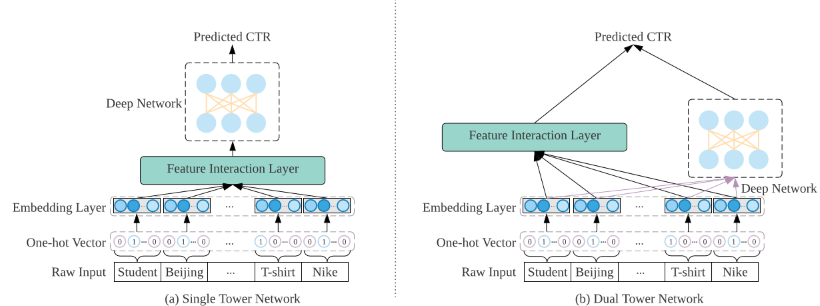
\includegraphics[width=\textwidth]{../figures/single_dual_dnn.png}
\caption{Deep Neural Network Architecture for CTR prediction. Image taken from \cite{RefWorks:zhang2021deep}}
\label{fig:dnn_architecture}
\end{figure}

Feature Interaction Operators can be categorized as either Product Operators, Convolutional Operators or 
Attention Operators. Product Operators such as the Product-based Neural Network (PNN) \citep{RefWorks:qu2016product-based}, 
Neural Factorization Machines (NFM) \citep{RefWorks:he2017neural}, Deep and Cross Network \citep{RefWorks:wang2017deep} and 
Gated Deep Cross Network (GDCN) \citep{RefWorks:wang2023deeper} introduce a product layer between the categorical 
feature embedding layer and the rest of the neural network in order to explicitly model the important feature 
interactions. Convolutional Operators such as the Convolutional Click Prediction Model (CCPM) \citep{RefWorks:liu2015convolutional} 
utilized convolution, pooling and non-linear activation in order to calculate arbitrary-order interactions. 
Finally, Attention Operators such as Attentional Factorization Machines (AFM) \citep{RefWorks:xiao2017attentional}, AutoInt 
\cite{RefWorks:song2019autoint} and Interpretable CTR prediction model with Hierarchical Attention (InterHAt) \citep{RefWorks:li2020interpretable}
utilize the attention mechanism to enable different feature interactions to contribute differently to the 
prediction.

\section{Deep Reinforcement Learning}

In their survey, \citep{RefWorks:wang2024deep} describe how deep reinforcement learning combines 
the aforementioned feature extraction capabilities of DNN’s with the decision-making 
capability of reinforcement learning, which aims to learn an optimal state-action policy 
which maximizes the expected reward gained in a given environment. In the context of 
recommendation systems, a significant amount of research has been dedicated to formulating 
the recommendation problem as a Contextual Multi-Armed Bandit (MAB) problem setting, where 
the context consists of user, site and item features \citep{RefWorks:bouneffouf2012contextual-bandit,RefWorks:li2010contextual-bandit,RefWorks:zeng2016online}. 
However, a shortcoming for the MAB approach 
is that it does not explicitly model the future expected reward for the policy, which may 
be detrimental in the longer term \citep{RefWorks:zheng2018drn:}. Markov Decision Process (MDP) models 
solve for this issue by modelling the state-action progression as a Markov Process, allowing 
for the stochastic valuation of the future potential rewards for a given recommendation 
policy \citep{RefWorks:lu2016partially,RefWorks:mahmood2007learning}. DRN \citep{RefWorks:zheng2018drn:} is a MDP framework 
that leverages a Deep Neural Network to approximate the expected total user response for 
each recommendation at each state. The two major advantages of DRN are firstly that it is 
composed on the basis of a continuous state and action representation, meaning that it can 
be scaled to large and sparse datasets, and secondly that the proposed reward function 
consists of both the immediate reward (user click) as well as the future expected reward 
(long term user engagement), thereby allowing for better recommendations over a user’s 
lifetime.

\chapter{Deep CTR model Evaluation}
\label{chap:deep-ctr-model-evaluation}

\section{Model Selection Methodology}

As explained above, I will explore a number of deep learning models. I selected five popular models on the basis of the following criteria

\begin{itemize}
\item Competitive predition accuracy in the KDD12, Criteo and Avazu datasets as published on Papers with Code.
\item Ideally, I was looking for a representitive set of models for each model type as discussed in (Zhang et. al. 2021). Therefore I was looking for models that employed Product Interaction Opetators, Attention Operators and Factorization Machines as a basis.
\item The code for the model has to be accessible and intuitive to use.
\end{itemize}

On the basis of the above critea, I have chosen the following models to explore:

\begin{itemize}
\item Factorization Supported Neural Networks
\item Product Based Neural Networks
\item Wide and Deep
\item DeepFM
\item Automatic Feature Interaction (AutoInt)
\end{itemize}

In the section below, I briefly introduce each of the models, and evaluate against the benchmark datasets loaded and preprocessed above.

\section{Model Summaries}

\subsection{Shallow Models}

\subsubsection{Logistic Regression}


\subsubsection{Factorization Machines}

Factorization Machines were first introduced in \citep{RefWorks:rendle2010factorization} as
a model class that ``combines the advantages of Support Vector Machines (SVM) with factorization models''.
The model is able to capture the second order feature interactions in the data, which is a key advantage over
Logistic Regression. The model is defined as follows:

\begin{equation}
\label{eq:fm}
\hat{y}(\mathbf{x}) = w_0 + \sum_{i=1}^{n} w_i x_i + \sum_{i=1}^{n} \sum_{j=i+1}^{n} \langle \mathbf{v}_i, \mathbf{v}_j \rangle x_i x_j
\end{equation}

where $w_0$ is the bias term, $w_i$ are the weights for the $i$-th feature, $\mathbf{v}_i$ are the latent vectors for the $i$-th feature.
\cite{RefWorks:rendle2010factorization} shows that the learned biases and weights of the FM model can be
computed in linear time, ``and can be learned efficiently by gradient descent methods'', such as Stochastic Gradient Descent (SGD).


\subsection{Deep Models}

\subsubsection{Factirization Supported Neural Networks}

The first Deep Learning model that we will consider is the Factorization Supported
Neural Network (FNN) model proposed by \cite{RefWorks:zhang2016deep}. The model works by first training a Factorization Machine
model on the sparse-encoded categorical input features. It then uses the latent vectors learned by the FM model (see $\mathbf{v}_i$ in equation~\ref{eq:fm})
as inputs to a Neural Network, as shown in Figure~\ref{fig:fnn}. In doing so, the FNN model is effectively using the FM latent factors to initialize the embedding layer of the Neural Network.
The DNN is then able to learn the higher order feature interactions in the data, which the FM model is unable to capture.

\begin{figure}[h]
\centering
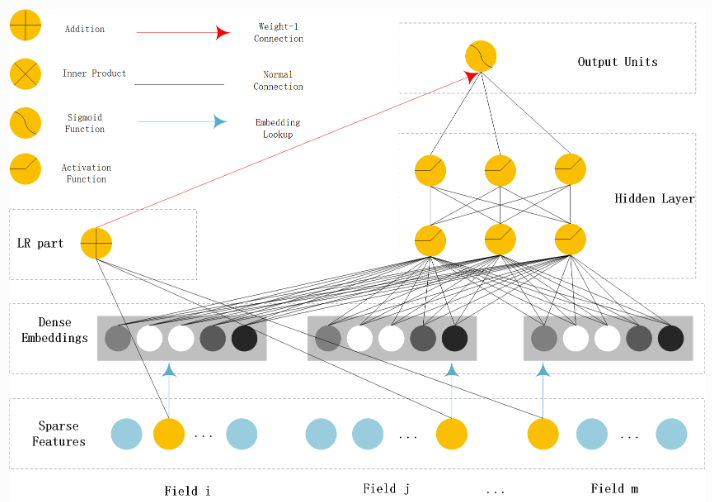
\includegraphics[]{../figures/fnn.png}
\caption{Factorization Supported Neural Network as proposed by \cite{RefWorks:zhang2016deep}. Image taken from \cite{RefWorks:shen2017deepctr:}}
\label{fig:fnn}
\end{figure}

\subsubsection{Product Based Neural Networks}

The Product Based Neural Network (PNN) model
proposed by \cite{RefWorks:qu2016product-based} is another Deep Learning
model that was developed around the same time as the FNN model. The key 
innovation of the PNN moel is the use of a pair-wisely connected Product Layer
after a field-wise connected embetting layer for the categorical features, as shown
in Figure~\ref{fig:pnn}. The Product Layer is able to directly model inter-field feature
interaction by means of either an inner product or outer production operation, and then further
distill higher feature inturactions by passing the output of the Product Layer through fully
connected MLP layers.


\begin{figure}[h]
\centering
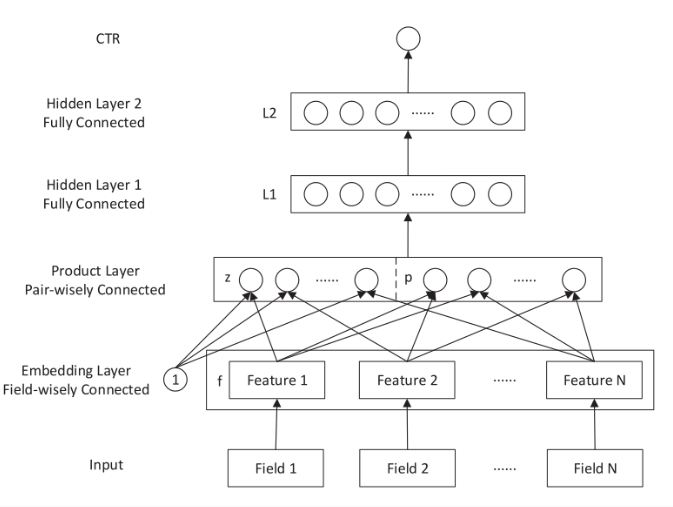
\includegraphics[]{../figures/pnn.png}
\caption{Product Based Neural Network as proposed by \cite{RefWorks:qu2016product-based}. Image taken from \cite{RefWorks:shen2017deepctr:}}
\label{fig:pnn}
\end{figure}


\subsubsection{Wide \& Deep Learning}

The Wide \& Deep Learning (WDL) model proposed by \cite{RefWorks:cheng2016wide} introduces the concept
of dual-tower model architecture \citep{RefWorks:zhang2021deep}. While both the FNN and the PNN models
generally tend to be constructed as a single fully connected DNN model, the Wide \& Deep model
consists of a wide component, consisting of a three layer Deep Neural Network that takes the concatinated
embedding vectors of the categorical features as input, and a deep component, consisting of a cross product
transformation of selected sparse categorical features. The logits from the wide and deep components are added
together to produce the final prediction. The architecture of the WDL model is shown in Figure~\ref{fig:wdl}.

\begin{figure}[h]
\centering
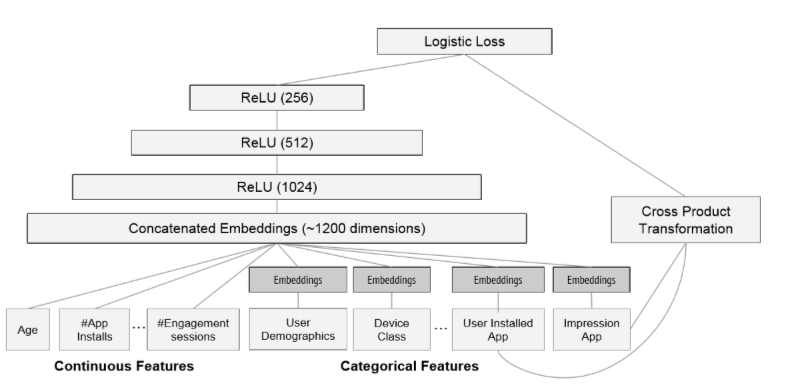
\includegraphics[]{../figures/wdl.png}
\caption{Wide \& Deep Learning model as proposed by \cite{RefWorks:cheng2016wide}}
\label{fig:wdl}
\end{figure}

The purpose behind the Dual-Tower architecture is to counteract the tendancy of the fully connected
single tower DNN models to lose the ability to capture low-order feature interactions \citep{RefWorks:zhang2021deep}.
The Wide component is able to capture the low-order feature interactions, while the Deep component is able to capture
the higher order feature interactions.

\subsubsection{DeepFM}

The DeepFM model proposed by \cite{RefWorks:guo2017deepfm:} can be thought of as an
imporvement of the aforementioned FNN \citep{RefWorks:zhang2016deep} and WDL \citep{RefWorks:cheng2016wide} models.
Like the FNN model, the DeepFM model usilises the Factorization Machine model \citep{RefWorks:rendle2010factorization}
to learn lower-order feature interactions. However, it also employs a dual-tower architecture
like the WDL model, with the Wide component being the FM model and the Deep component being a fully connected
DNN model. The DeepFM model is therefore able to avoid the limitations on capturing low-order
interactions that are inherent in the FNN model. In addition, due the the application of the FM to all
feature embeddings, the DeepFM model eliminates the need to choose which features 
to feed through the wide component, as is the case in the WDL model. The architecture of the DeepFM model is shown 
in Figure~\ref{fig:deepfm}.

\begin{figure}[h]
\centering
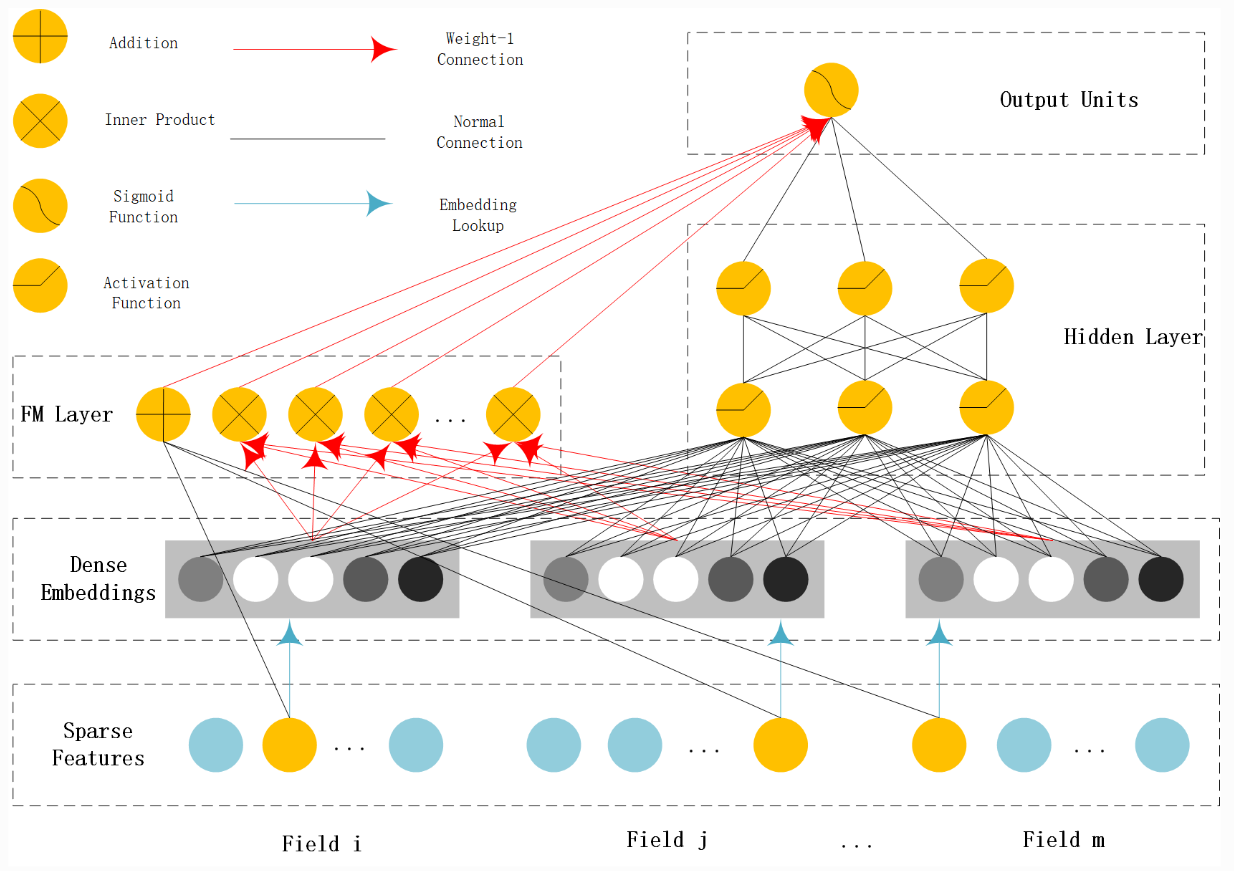
\includegraphics[width=\textwidth]{../figures/dfm.png}
\caption{DeepFM model as proposed by \cite{RefWorks:guo2017deepfm:}. Image taken from \cite{RefWorks:shen2017deepctr:}}
\label{fig:deepfm}
\end{figure}

%\subsubsection{Feature Generation by Convolutional Neural Network}

\subsubsection{Automatic Feature Interaction Learning}

The Autotomatic Feature Interaction Learning (AutoInt) model proposed by
\cite{RefWorks:song2019autoint} makes use of a multi-head self attention
network to model the important feature interactions in the data. The initial 
paper separates the model into three parts: an embedding layer, an interaction layer 
and an output layer. The embedding layer aims to project each sparse multi-value
categorical a and dense numerical feature into a lower dimensional space, as per the equation~\ref{eq:autoint-embedding}:

\begin{equation}
\label{eq:autoint-embedding}
\mathbf{e_i} = \frac{1}{q} \mathbf{V_i x_i}
\end{equation}

where $\mathbf{V_i}$ is the embedding matrix for the $i$-th field, $x_i$ is a multi-hot vector, and $q$ 
is the number of non-zero values in $x_i$. The interaction layer employs the multi-head
mechanism to determine which higher order feature interaction are meaningful in the data. This not only
improves the efficiency of model traning, but it also improves the model's explainability. Lastly,
the output layer is a fully connected layer that takes in the concatinated output 
of the interaction layer, and applies the sigmoid activation function to produce the final prediction.
The architecture of the AutoInt model is shown in Figure~\ref{fig:autoint}.

\begin{figure}[h]
\centering
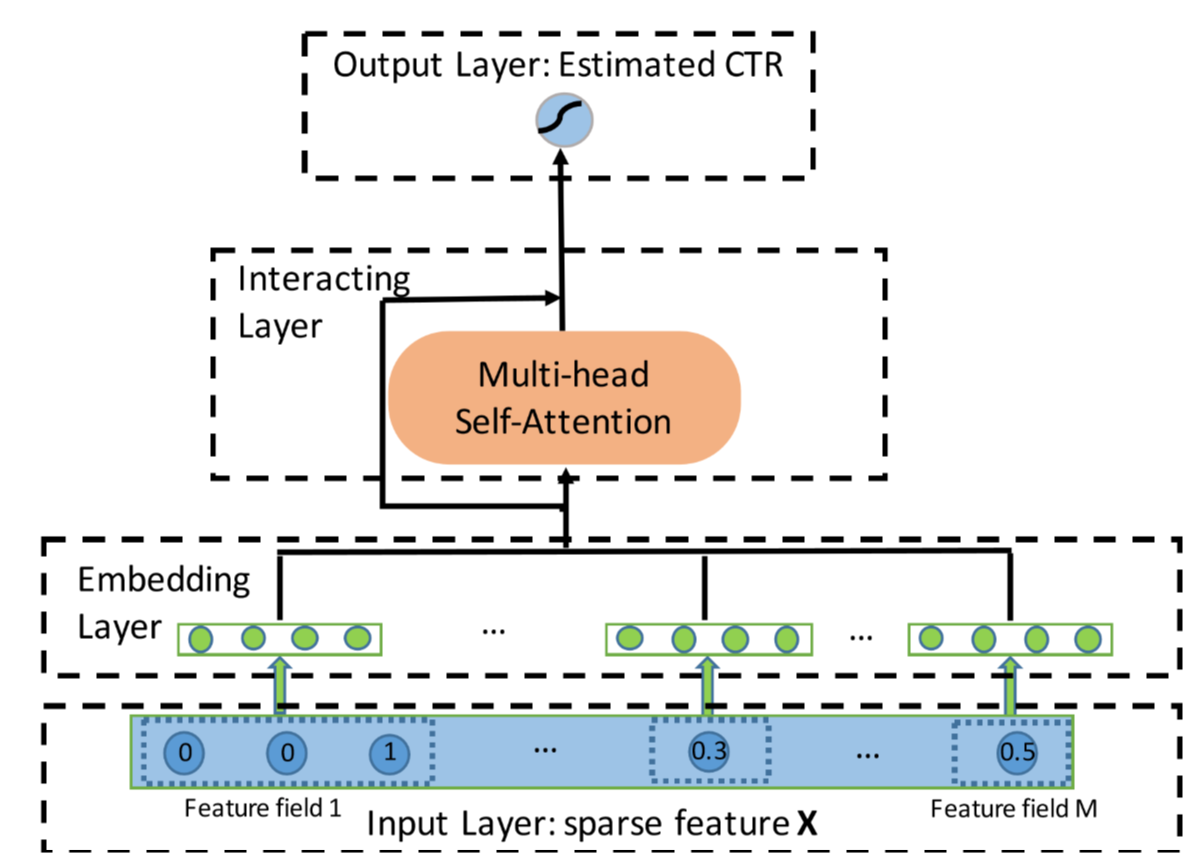
\includegraphics[width=\textwidth]{../figures/autoint.png}
\caption{AutoInt model as proposed by \cite{RefWorks:song2019autoint}}
\label{fig:autoint}
\end{figure}

\section{Benchmark Datasets and Exploratory Data Analysis}

\section{Model Evaluation}

\section{Deep CTR Model Results}

\chapter{Deep Reinforcement Learning for Ad Personalization}
\label{chap:deep-rl-for-ad-personalization}

\section{DeepCTR-RL Framework}

\section{Experiment Setup}

\section{Results}

\chapter{Discussion}
\label{chap:discussion}

Discussion goes here.

\chapter{Conclusion}


Conclusion goes here. 





\clearpage
 %% reset page counter and start appendix pages with A
\pagenumbering{arabic}
\renewcommand*{\thepage}{A\arabic{page}}

%% Appendix goes here
%\appendix
%
%\chapter{Appendix title}
%
%Appendix goes here.


%%References part of appendices
% References: modify the file refs.bib
\bibliographystyle{plainnat}
\bibliography{refs}


\end{document}
